\chapter{Analysis}

\qquad The final output of the PPar tool \ref{ppar-tool} has been transformed into the tabular format shown in the figure \ref{analysis-data-table} below. The table contains all loops (roughly 1400) from NAS benchmarks. PPar tool computed metric vectors for all the loops. All loops have been labelled as parallelisible or not with the help of Intel ICC compiler, which performs the role of expert-opinion in this project. 

\begin{figure}[htb]
	\centering
	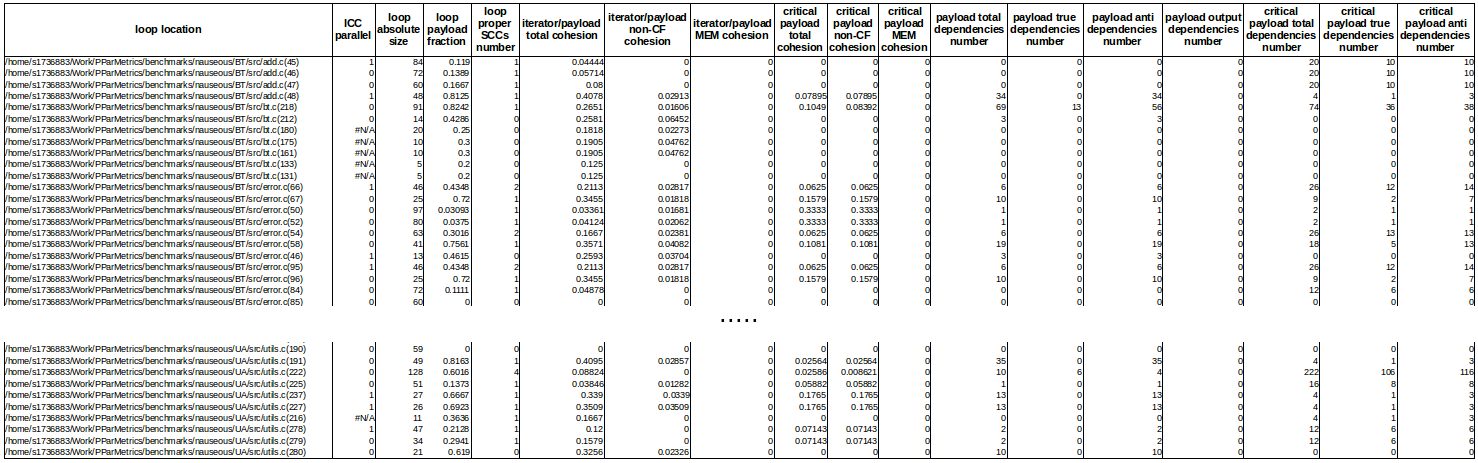
\includegraphics[width=\linewidth]{figs/metrics-table.png}
	\caption{Analysis input table with computed metrics and ICC parallelizability classification labels.}
	\label{analysis-data-table}
\end{figure}
  
This table has been used as an input to different sorts of statistical learning and analysis methods as well as for manual human analysis. 

\section{Visual data representations}
\qquad The first step in the analysis of collected loop metrics and parallelisability properties is to visualize the data and manually check for existent data patterns and correlations. Python packages pandas \cite{python-lib-pandas} and matplotlib \cite{python-matplotlib} have been used for the task. 


\section{Statistical analysis}

\qquad Statistical analysis of loop parallelisability metrics has been conducted with the help of pandas \cite{python-lib-pandas} and scikit-learn \cite{python-lib-scikit-learn} python packages. Detailed description of all algorithms, techniques and all underlying mathematical foundations can be found in the introduction to statistical analysis book \cite{statistical-learning-book}.

\subsection{K-Means clustering}

\qquad In this work k-means clustering techniques have been used as the first method of statistical analysis.




\subsection{SVM-based parallelisability analyzer}

\section{Manual analysis}